\documentclass[conf]{new-aiaa}
%\documentclass[journal]{new-aiaa} %for journal papers
%\documentclass[a4paper]{article}
%\documentclass{homework}

%% Sets page size and margins
%\usepackage[a4paper,top=3cm,bottom=2cm,left=3cm,right=3cm,marginparwidth=0.8.75cm]{geometry}

%\usepackage[utf8]{inputenc}
\usepackage{graphicx}
\usepackage{amsmath}
\usepackage[version=4]{mhchem}
\usepackage{siunitx}
\usepackage{longtable,tabularx}
\setlength\LTleft{0pt} 
%======================================

% additions
\graphicspath{ {figures/} }
\usepackage{floatrow}
\usepackage{ar}
\usepackage{amstext} % for \text macro
\usepackage{array}   % for \newcolumntype macro
\usepackage{gensymb} % for degree symbol
\newcolumntype{L}{>{$}l<{$}} % math-mode version of "l" column type
\usepackage[numbered,framed]{matlab-prettifier}
\usepackage{fancyvrb}

\pagestyle{empty}

\definecolor{listinggray}{gray}{0.9}
\definecolor{lbcolor}{rgb}{0.9,0.9,0.9}
\lstset{
backgroundcolor=\color{lbcolor},
    tabsize=4,    
%   rulecolor=,
    language=fortran,
        basicstyle=\mlttfamily,
        upquote=true,
        aboveskip={1.5\baselineskip},
        columns=fixed,
        showstringspaces=false,
        extendedchars=false,
        breaklines=true,
        prebreak = \raisebox{0ex}[0ex][0ex]{\ensuremath{\hookleftarrow}},
        frame=single,
        numbers=left,
        showtabs=false,
        showspaces=false,
        showstringspaces=false,
        identifierstyle=\mlttfamily,
				keywordstyle=\color{blue}\mlttfamily,
				stringstyle=\color{red}\mlttfamily,
				commentstyle=\color[RGB]{34,139,34}\mlttfamily,
				morecomment=[l][\color{magenta}]{\#}
        %keywordstyle=\color[rgb]{0,0,1},
        %commentstyle=\color[rgb]{0.026,0.112,0.095},
        %stringstyle=\color[rgb]{0.627,0.126,0.941},
        %numberstyle=\color[rgb]{0.205, 0.142, 0.73},
%        \lstdefinestyle{C++}{language=C++,style=numbers}’.
}
%\usepackage{titlesec}
%\titleformat*{\paragraph}{\large\bfseries}
%======================================
\title{CE 791 HPC - Final Exam}

\author{Andrew Navratil}

\begin{document}

\maketitle

\section*{Problem 3: Simpson's Rule Integration}

\begin{figure}[H]
	\centering
	\begin{floatrow}
		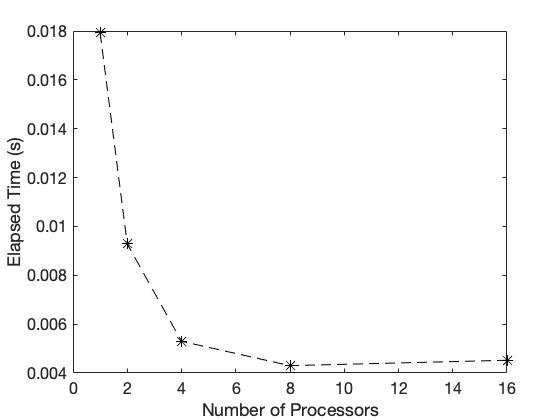
\includegraphics[width=.5\columnwidth]{../finaldata/times_p3.jpg}
		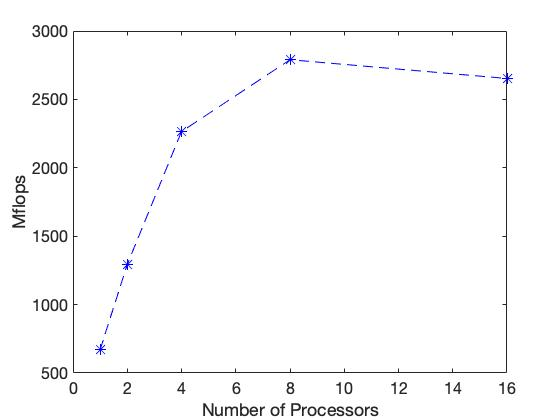
\includegraphics[width=.5\columnwidth]{../finaldata/mflops_p3.jpg}
	\end{floatrow}
	\caption{Execution Times, Mflops for Problem 3}
\end{figure}

Benchmarking plots show an increase in mflops and decrease in execution time for this parallel implementation up through the use of 8 processors, however using 16 showed a decrease from 8.  Explanation for this decrease is unknown, perhaps it is due to the use of 2 MPI\_REDUCE calls and that causes too much parallel communication overhead at 16 procs.

\section*{Problem 4: Sum 1-p}

\begin{figure}[H]
	\centering
	\begin{floatrow}
		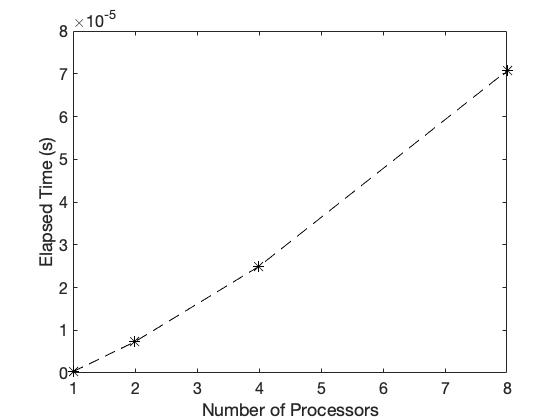
\includegraphics[width=.5\columnwidth]{../finaldata/times_p4.jpg}
		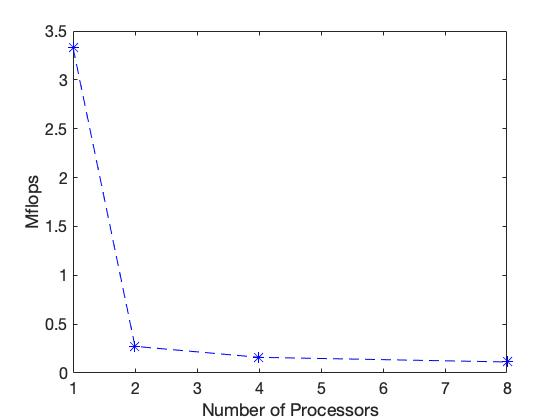
\includegraphics[width=.5\columnwidth]{../finaldata/mflops_p4.jpg}
	\end{floatrow}
	\caption{Execution Times, Mflops for Problem 4}
\end{figure}

Testing the parallel sum code, summing 1 to num procs p, shows a decrease in Mflops and increase in execution times as num procs increases.  This is likely due to the simplicity of the simple single addition/assignment for each processor, so parallel communication overhead is the biggest issue for parallel scalability on this problem.

\section*{Problem 5: 6-digit conditional combinations}

Parallel code was written for a specific number of processors for this problem, that being 9, where each processor performed calculations for a combination with the starting digit being the processor number plus one.  The total number of combinations was calculated as 527787.

\section*{Problem 7: 1D GW Flow with v2 Jacobi, RBGS, OpenMP}

\begin{figure}[H]
	\centering
	\begin{floatrow}
		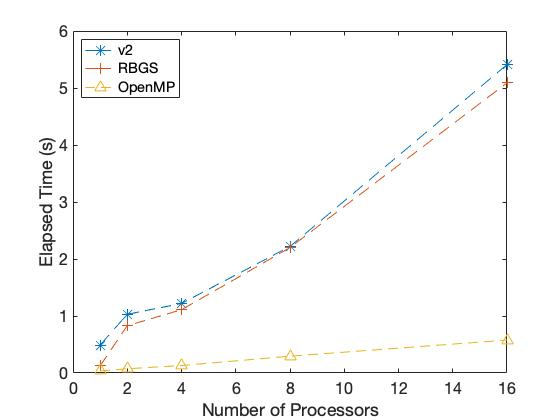
\includegraphics[width=.5\columnwidth]{../finaldata/times_p7.jpg}
		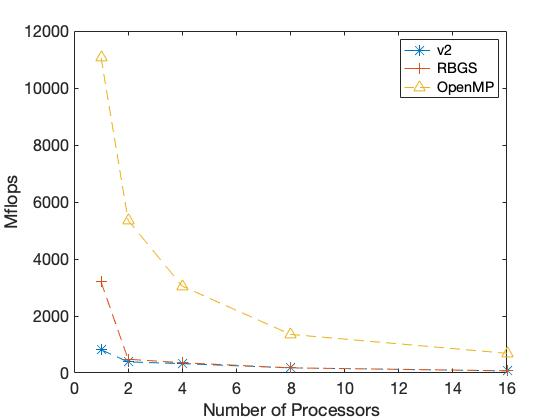
\includegraphics[width=.5\columnwidth]{../finaldata/mflops_p7.jpg}
	\end{floatrow}
	\caption{Execution Times, Mflops for Problem 7}
\end{figure}

Benchmarking plots again show an increase in mflops and decrease in execution time for this parallel implementation up through the use of all 16 processors.  The cause for drop in performance is still unknown.  The OpenMP version achieved significantly better performance than MPI Red-Black Gauss-Seidel or MPI Jacobi v2.  The accuracy (solution error) for Jacobi was $0.0101$ and for both the MPI and OpenMP versions of RBGS it was $0.0196$.

\newpage
\section*{Problem 9: Containment Source}

\begin{figure}[H]
	\centering
	\begin{floatrow}
		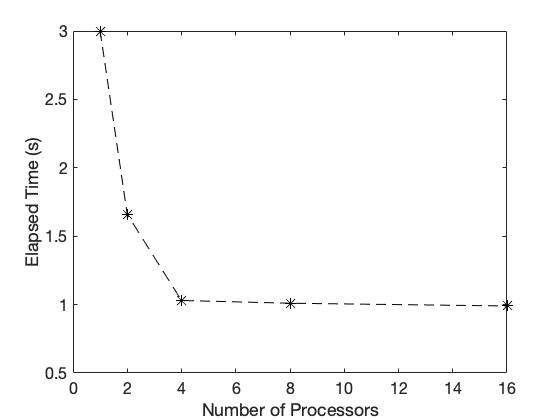
\includegraphics[width=.5\columnwidth]{../finaldata/times_p9.jpg}
	\end{floatrow}
	\caption{Execution Times for Problem 9}
\end{figure}

Parallel random search was implemented for combinations of x0,y0 and M0, using integer values in the respective ranges.  MPI\_MINLOC was utilized with MPI\_ALLREDUCE in order to get the processor finding the minimum least squares difference between the observed and calculated values.  MPI\_GATHER was then used to get the actual values of min x0,y0,M0.  Note that observation values in the pdf are assumed to have been printed like a typical x-y grid with origin in bottom left, so top y row is 400m and bottom y row is 0m.

Benchmarking the execution times shows the expected decrease as number of processors increases, with the largest drop seen up to 4, with slight improvements using 8 or 16.

The optimized combinations were different on each run, presumably due to the amount of possible combinations there are (1e6 number of random combinations was tried on each run).  Runs were also executed with 1e8 trials, and still produced different combinations.  The values received for each final run of num procs at 1e6 trials is:

\bigskip
\begin{tabular}{ |c|c|c|c| } 
 \hline
	\text{Num Procs} & x0 & y0 & M0 \\ 
 \hline
	1 & 836 & 299 & 36 \\
 \hline
	2 & 791 & 203 & 77 \\
 \hline
	4 & 335 & 194 & 21 \\
 \hline
	8 & 342 & 204 & 74 \\
 \hline
	16 & 589 & 343 & 35 \\
 \hline
\end{tabular}

%======================================
\newpage

\section*{Fortran Code: Problem 3}
\lstinputlisting[language=fortran]{../p3.f90}
\newpage

\section*{Fortran Code: Problem 4}
\lstinputlisting[language=fortran]{../p4.f90}
\newpage

\section*{Fortran Code: Problem 5}
\lstinputlisting[language=fortran]{../p5.f90}
\newpage

\section*{Fortran Code: Problem 7 v2}
\lstinputlisting[language=fortran]{../jacobiv2.f90}
\newpage

\section*{Fortran Code: Problem 7 RBGS}
\lstinputlisting[language=fortran]{../jacobigs.f90}
\newpage

\section*{Fortran Code: Problem 7 OpenMP}
\lstinputlisting[language=fortran]{../jacobiopenmp.f90}
\newpage

\section*{Fortran Code: Problem 9}
\lstinputlisting[language=fortran]{../p9.f90}
\newpage

\section*{Matlab Code}

\lstset{
  style      = Matlab-editor,
  basicstyle = \mlttfamily,
}
\lstinputlisting{../final.m}

\end{document}

